%% BioMed_Central_Tex_Template_v1.06
%%                                      %
%  bmc_article.tex            ver: 1.06 %
%                                       %

%%IMPORTANT: do not delete the first line of this template
%%It must be present to enable the BMC Submission system to
%%recognise this template!!

%%%%%%%%%%%%%%%%%%%%%%%%%%%%%%%%%%%%%%%%%
%%                                     %%
%%  LaTeX template for BioMed Central  %%
%%     journal article submissions     %%
%%                                     %%
%%          <8 June 2012>              %%
%%                                     %%
%%                                     %%
%%%%%%%%%%%%%%%%%%%%%%%%%%%%%%%%%%%%%%%%%


%%%%%%%%%%%%%%%%%%%%%%%%%%%%%%%%%%%%%%%%%%%%%%%%%%%%%%%%%%%%%%%%%%%%%
%%                                                                 %%
%% For instructions on how to fill out this Tex template           %%
%% document please refer to Readme.html and the instructions for   %%
%% authors page on the biomed central website                      %%
%% http://www.biomedcentral.com/info/authors/                      %%
%%                                                                 %%
%% Please do not use \input{...} to include other tex files.       %%
%% Submit your LaTeX manuscript as one .tex document.              %%
%%                                                                 %%
%% All additional figures and files should be attached             %%
%% separately and not embedded in the \TeX\ document itself.       %%
%%                                                                 %%
%% BioMed Central currently use the MikTex distribution of         %%
%% TeX for Windows) of TeX and LaTeX.  This is available from      %%
%% http://www.miktex.org                                           %%
%%                                                                 %%
%%%%%%%%%%%%%%%%%%%%%%%%%%%%%%%%%%%%%%%%%%%%%%%%%%%%%%%%%%%%%%%%%%%%%

%%% additional documentclass options:
%  [doublespacing]
%  [linenumbers]   - put the line numbers on margins

%%% loading packages, author definitions

%\documentclass[twocolumn]{bmcart}% uncomment this for twocolumn layout and comment line below
\documentclass[doublespacing]{bmcart}

%%% Load packages
\usepackage{amsthm,amsmath}
%\RequirePackage{natbib}
%\RequirePackage[authoryear]{natbib}% uncomment this for author-year bibliography
\RequirePackage{hyperref}
%\usepackage[utf8]{inputenc} %unicode support
\usepackage[applemac]{inputenc} %applemac support if unicode package fails
%\usepackage[latin1]{inputenc} %UNIX support if unicode package fails
\usepackage{subcaption}


%%%%%%%%%%%%%%%%%%%%%%%%%%%%%%%%%%%%%%%%%%%%%%%%%
%%                                             %%
%%  If you wish to display your graphics for   %%
%%  your own use using includegraphic or       %%
%%  includegraphics, then comment out the      %%
%%  following two lines of code.               %%
%%  NB: These line *must* be included when     %%
%%  submitting to BMC.                         %%
%%  All figure files must be submitted as      %%
%%  separate graphics through the BMC          %%
%%  submission process, not included in the    %%
%%  submitted article.                         %%
%%                                             %%
%%%%%%%%%%%%%%%%%%%%%%%%%%%%%%%%%%%%%%%%%%%%%%%%%


\def\includegraphic{}
\def\includegraphics{}


\usepackage{todonotes}
\usepackage{multirow}
%%% Put your definitions there:
\startlocaldefs
\newcommand{\pv}{\textit{P. vivax}}
\newcommand{\pf}{\textit{P. falciparum}}
\newcommand{\males}{M15$+$}
\graphicspath{{../figures/}}
\endlocaldefs


%%% Begin ...
\begin{document}

%%% Start of article front matter
\begin{frontmatter}

\begin{fmbox}
\dochead{Research}

%%%%%%%%%%%%%%%%%%%%%%%%%%%%%%%%%%%%%%%%%%%%%%
%%                                          %%
%% Enter the title of your article here     %%
%%                                          %%
%%%%%%%%%%%%%%%%%%%%%%%%%%%%%%%%%%%%%%%%%%%%%%

\title{Assessing a 2020--2025 primaquine intervention in Cambodia to control vivax malaria}

%%%%%%%%%%%%%%%%%%%%%%%%%%%%%%%%%%%%%%%%%%%%%%
%%                                          %%
%% Enter the authors here                   %%
%%                                          %%
%% Specify information, if available,       %%
%% in the form:                             %%
%%   <key>={<id1>,<id2>}                    %%
%%   <key>=                                 %%
%% Comment or delete the keys which are     %%
%% not used. Repeat \author command as much %%
%% as required.                             %%
%%                                          %%
%%%%%%%%%%%%%%%%%%%%%%%%%%%%%%%%%%%%%%%%%%%%%%

%\author[
%   addressref={aff1},                   % id's of addresses, e.g. {aff1,aff2}
%   corref={aff1},                       % id of corresponding address, if any
%   noteref={n1},                        % id's of article notes, if any
%   email={jane.e.doe@cambridge.co.uk}   % email address
%]{\inits{JE}\fnm{Jane E} \snm{Doe}}
%\author[
%   addressref={aff1,aff2},
%   email={john.RS.Smith@cambridge.co.uk}
%]{\inits{JRS}\fnm{John RS} \snm{Smith}}
\author[
   addressref={bi},
   email={rowan.martin-hughes@burnet.edu.au}
]{\inits{R}\fnm{Rowan} \snm{Martin-Hughes}}
%
\author[
   addressref={bi,melbms,melbph},                   % id's of addresses, e.g. {aff1,aff2}
   %corref={aff1},                       % id of corresponding address, if any
   %noteref={n1},                        % id's of article notes, if any
   email={r.hickson@UNSWalumni.com}   % email address
]{\inits{RI}\fnm{RI} \snm{Hickson}}
%
\author[
   addressref={menzies},
   email={angela.devine@menzies.edu.au}
]{\inits{A}\fnm{Angela} \snm{Devine}}
%
\author[
   addressref={melbph,doherty},
   email={david.price1@unimelb.edu.au}
]{\inits{DJ}\fnm{David J} \snm{Price}}
\author[
   addressref={menzies},
   email={kamala.ley-thriemer@menzies.edu.au}
]{\inits{K}\fnm{Kamala} \snm{Thriemer}}
%
% from here, excepting senior, authors are alphabetical
\author[
   addressref={bi},
   email={freya.fowkes@burnet.edu.au}
]{\inits{FJI}\fnm{Freya JI} \snm{Fowkes}}
%
\author[
   addressref={melbms,melbph,doherty},
   email={jamesm@unimelb.edu.au}
]{\inits{JM}\fnm{James M} \snm{McCaw}}
%
\author[
   addressref={melbph},
   email={julieas@unimelb.edu.au}
]{\inits{JA}\fnm{Julie A} \snm{Simpson}}
%
\author[
   addressref={cnm},
   email={sivsovannaroths@gmail.com}
]{\inits{S}\fnm{Siv} \snm{Sovannaroth}}
%
\author[
   addressref={cnm,moru},
   email={pengby@email.com}
]{\inits{P}\fnm{Pengby} \snm{Ngor}}

%%%%%%%%%%%%%%%%%%%%%%%%%%%%%%%%%%%%%%%%%%%%%%
%%                                          %%
%% Enter the authors' addresses here        %%
%%                                          %%
%% Repeat \address commands as much as      %%
%% required.                                %%
%%                                          %%
%%%%%%%%%%%%%%%%%%%%%%%%%%%%%%%%%%%%%%%%%%%%%%

%\address[id=aff1]{%                           % unique id
%  \orgname{Department of Zoology, Cambridge}, % university, etc
%  %\street{Waterloo Road},                     %
%  %\postcode{}                                % post or zip code
%  \city{London},                              % city
%  \cny{UK}                                    % country
%}
%\address[id=aff2]{%
%  \orgname{Marine Ecology Department, Institute of Marine Sciences Kiel},
%  %\street{D\"{u}sternbrooker Weg 20},
%  %\postcode{24105}
%  \city{Kiel},
%  \cny{Germany}
%}
\address[id=bi]{%
  \orgname{Burnet Institute},
  %\street{},
  %\postcode{24105}
  \city{Melbourne},
  \cny{Australia}
}
\address[id=melbms]{%                           % unique id
  \orgname{School of Mathematics and Statistics, Faculty of Science, University of Melbourne}, % university, etc
  %\street{},                     %
  %\postcode{}                                % post or zip code
  \city{Parkville},                              % city
  \cny{Australia}                                    % country
}
\address[id=melbph]{%
  \orgname{Melbourne School of Population and Global Health, Faculty of Medicine, Dentistry, and Health Sciences, University of Melbourne}, % university, etc
  %\street{},                     %
  %\postcode{}                                % post or zip code
  \city{Parkville},                              % city
  \cny{Australia}                                    % country
}

\address[id=menzies]{%
  \orgname{Menzies School of Health Research},
  %\street{},
  %\postcode{24105}
  \city{Melbourne},
  \cny{Australia}
}
\address[id=doherty]{%
  \orgname{Doherty Institute},
  %\street{},
  %\postcode{24105}
  \city{Melbourne},
  \cny{Australia}
}
\address[id=cnm]{%
  \orgname{Cambodian National Center for Parasitology, Entomology and Malaria Control},
  %\street{},
  %\postcode{24105}
  \city{Phnom Penh},
  \cny{Cambodia}
}
\address[id=moru]{%
  \orgname{Mahidol-Oxford Tropical Medicine Research Unit, Faculty of Tropical Medicine, Mahidol University},
  %\street{},
  %\postcode{24105}
  \city{Bangkok},
  \cny{Thailand}
}

%%%%%%%%%%%%%%%%%%%%%%%%%%%%%%%%%%%%%%%%%%%%%%
%%                                          %%
%% Enter short notes here                   %%
%%                                          %%
%% Short notes will be after addresses      %%
%% on first page.                           %%
%%                                          %%
%%%%%%%%%%%%%%%%%%%%%%%%%%%%%%%%%%%%%%%%%%%%%%

\begin{artnotes}
%\note{Sample of title note}     % note to the article
%\note[id=n1]{Equal contributor} % note, connected to author
\end{artnotes}

\end{fmbox}% comment this for two column layout

%%%%%%%%%%%%%%%%%%%%%%%%%%%%%%%%%%%%%%%%%%%%%%
%%                                          %%
%% The Abstract begins here                 %%
%%                                          %%
%% Please refer to the Instructions for     %%
%% authors on http://www.biomedcentral.com  %%
%% and include the section headings         %%
%% accordingly for your article type.       %%
%%                                          %%
%%%%%%%%%%%%%%%%%%%%%%%%%%%%%%%%%%%%%%%%%%%%%%

\begin{abstractbox}
% Instructions from: https://malariajournal.biomedcentral.com/submission-guidelines/preparing-your-manuscript/research-article
%Abstract
%The Abstract should not exceed 350 words. Please minimize the use of abbreviations and do not cite references in the abstract. Reports of randomized controlled trials should follow the CONSORT extension for abstracts. The abstract must include the following separate sections:
%
%Background: the context and purpose of the study
%Methods: how the study was performed and statistical tests used
%Results: the main findings
%Conclusions: brief summary and potential implications
%Trial registration: If your article reports the results of a health care intervention on human participants, it must be registered in an appropriate registry and the registration number and date of registration should be in stated in this section. If it was not registered prospectively (before enrollment of the first participant), you should include the words 'retrospectively registered'. See our editorial policies for more information on trial registration

\begin{abstract} % abstract

\parttitle{Background} %the context and purpose of the study
Elimination targets for \textit{Plasmodium vivax} are approaching, with the Cambodian target 2025. Quantitative tools can help determine if proposed new strategies will be sufficient to meet those targets.

\parttitle{Methods} %how the study was performed and statistical tests used
We calibrated the Optima malaria transmission model reported case data from 2011--2018 for six provinces with different transmission levels. The model had two human populations: with males 15 years plus, and everyone else. We used the calibrated model to explore for best and worst case interpretations of the available case data, and of the primaquine intervention.

\parttitle{Results} %the main findings
We found elimination is unlikely to be reached in provinces with fairly high burdens of \textit{Plasmodium vivax}, such as Pursat, by only targeting adult males with primaquine. However, it will substantially reduce transmission. As such, we identify how many tests will need to be conducted to have 99\% confidence of detecting at least one case, given the lower incidence by 2025.
%\todo[inline]{We don't need to detect a positive case, should this be rephrased or related to an elimination target? Maybe add something quantitative about how much incidence/prevalence/mortality could be reduced under the best/worse case scenarios?}

\parttitle{Conclusions}
A primaquine intervention targeting adult males is likely to have a substantial impact on transmission of \pv, though it is not projected to result in elimination from all provinces by the 2025 target even under the most optimistic interpretation of the available case data. 
%The surveillance requirements to ensure the resulting lower incidence is detected as Cambodia approaches elimination may be infeasible in provinces such as Takeo that already have low incidence of \pv, especially as all provinces will see a decrease in case counts as the intervention is nationwide.
%\todo[inline]{Consider additional conclusion around surveillance and elimination?}

\end{abstract}

%%%%%%%%%%%%%%%%%%%%%%%%%%%%%%%%%%%%%%%%%%%%%%
%%                                          %%
%% The keywords begin here                  %%
%%                                          %%
%% Put each keyword in separate \kwd{}.     %%
%%                                          %%
%%%%%%%%%%%%%%%%%%%%%%%%%%%%%%%%%%%%%%%%%%%%%%

\begin{keyword}
\kwd{Malaria}
\kwd{\textit{Plasmodium vivax}}
\kwd{Transmission}
\kwd{Primaquine}
\kwd{Radical cure}
\kwd{Mathematical model}
\end{keyword}

% MSC classifications codes, if any
%\begin{keyword}[class=AMS]
%\kwd[Primary ]{}
%\kwd{}
%\kwd[; secondary ]{}
%\end{keyword}

\end{abstractbox}
%
%\end{fmbox}% uncomment this for twcolumn layout

\end{frontmatter}

%%%%%%%%%%%%%%%%%%%%%%%%%%%%%%%%%%%%%%%%%%%%%%
%%                                          %%
%% The Main Body begins here                %%
%%                                          %%
%% Please refer to the instructions for     %%
%% authors on:                              %%
%% http://www.biomedcentral.com/info/authors%%
%% and include the section headings         %%
%% accordingly for your article type.       %%
%%                                          %%
%% See the Results and Discussion section   %%
%% for details on how to create sub-sections%%
%%                                          %%
%% use \cite{...} to cite references        %%
%%  \cite{koon} and                         %%
%%  \cite{oreg,khar,zvai,xjon,schn,pond}    %%
%%  \nocite{smith,marg,hunn,advi,koha,mouse}%%
%%                                          %%
%%%%%%%%%%%%%%%%%%%%%%%%%%%%%%%%%%%%%%%%%%%%%%

%%%%%%%%%%%%%%%%%%%%%%%%% start of article main body
% <put your article body there>

%%%%%%%%%%%%%%%%
%% Background %%
%%
%Instructions for authors from: https://malariajournal.biomedcentral.com/submission-guidelines/preparing-your-manuscript/research-article
%Background
%The Background section should explain the background to the study, its aims, a summary of the existing literature and why this study was necessary or its contribution to the field.
\section*{Background} 

\textit{Plasmodium vivax} (\pv) is the cause of a significant burden of malaria globally, with an estimated 14.3 million cases in 2017~\cite{Battle2019}. With the rise of artemisinin-resistant \textit{Plasmodium falciparum} in Cambodia, the relative burden of \pv~has increased due to increased focus on eliminating \pf. Vivax malaria is now responsible for 30--80\% of cases across the provinces in Cambodia~\cite{Pengby, Sandfort2020}. The key difference between \pf~and \pv~is the hypnozoite stage of \pv, which results in relapses~\cite{Douglas2013, Commons2019}. Targeting the hypnozoite reservoir is key since an estimated 79\% of \pv~episodes are due to relapses \cite{Commons2020}.   

Standard treatment for \pv~in Cambodia is chloroquine (CQ) for the blood stage infection. In addition to the blood-stage treatment, radical cure is needed to clear the hypnozoites. The only widely available drug for radical cure is primaquine (PQ). The WHO recommendation is to test for G6PD deficiency before administration of PQ in order to avoid the primaquine-induced hemolysis that can result in those with this enzymopathy~\cite{WHO2015malaria}. G6PD deficiency is measured by enzymatic activity and the cut off for normal activity is 30\%. Since G6PD deficiency is x-linked, females may be homozygous or heterozygous. The latter is more challenging to detect as some will have $>$30\% activity but still be at risk of severe hemolysis \cite{Chu2017}. 

The elimination target for \pv~in Cambodia is 2025~\cite{Cambodia}. Cambodia is currently trialling the use of a 14-day low-dose primaquine intervention for adult males testing G6PD normal with ? test in two health centres in Pursat province\todo{Check if this is still the situation or if it needs to be rephrased, add detail on what kind of test is conducted}. If successful, this will be expanded into the national programme. We use transmission modelling to determine if this is likely to be sufficient to eliminate \pv~by the 2025 target. 

%Methods
%The methods section should include:
%
%the aim, design and setting of the study
%the characteristics of participants or description of materials
%a clear description of all processes, interventions and comparisons. Generic drug names should generally be used. When proprietary brands are used in research, include the brand names in parentheses
%the type of statistical analysis used, including a power calculation if appropriate
\section*{Methods} \label{sec:methods} %Subsections are currently modelled on Scott et al. 2017

\subsection*{Data sources and synthesis} 
Demographic data, including mortality, were obtained from the National Institute of Statistics in Cambodia~\ref{}. Data on malaria incidence were obtained from the Cambodia National Center for Parasitology, Entomology and Malaria Control (CNM)~\ref{CNM_Pengby}.

The raw data included total number of tests, and numbers of positive tests by parasite species, test type, province, and week of test. The population stratification for \pv~incidence was provided as a proportion of cases by age and sex, from 2015--2019. Therefore, data for each province was pro-rated to achieve the correct proportion of cases for males 15 years and older. 

%\item Some provinces (list)\todo{check with RIH on original data files? Is this valid - in the model calibration section it says that provinces where the border has changed were excluded?} were combined to maintain static borders across the data period of 2011--2018. 

%The aggregated data used for model calibration are provided in Additional file~\ref{supp}.

\subsection*{Epidemic model}

The dynamic transmission model of \pv~is based on that by Scott~\etal~\cite{scott2017}. It accounts for transmission between humans and mosquitoes, with the conceptual disease progression in the model depicted in Fig~\ref{fig:model_flow}. People in the model are identified as: susceptible; infected with \pv~in the liver only (hypnozoites and/or active liver stage); infected with active blood stage infection able to infect mosquitoes (gametocytes present -- further divided into clinical, severe, or asymptomatic); or recovered and immune (with no hypnozoites). The recovered and immune compartment is important for capturing \pv~dynamics given our current understanding of the importance of immunity in reducing transmission or symptomatic infections~\cite{}\todo{AD: fact check me}. The human population is stratified into males 15 years and older (M15+) and everyone else (Gen), to enable the primaquine intervention proposed in Cambodia to be captured by the model. Further details on the full model structure, parameter values, and calibration are provided in Additional file~\ref{supp}.

\begin{figure}[h!]
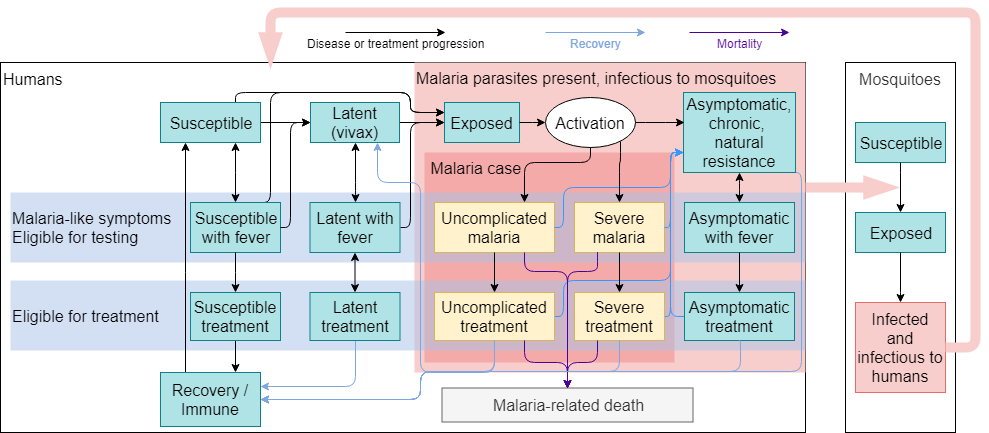
\includegraphics[width=.95\linewidth]{Optima_Malaria_model_diagram.png}\label{fig:model_flow}\caption{\csentence{Optima Malaria model diagram}}
\end{figure}


\subsection*{Model calibration} \label{sec:calibration} % and validation 

Data on annual incidence (2011--2018), testing numbers, and demographics were used to calibrate the model for each population stratification (i.e. males 15 years and over, and everyone else) and province (see Additional file~\ref{supp}). 

The population size was modelled in each province by group, including transitions from the general population (Gen) to adult males (M15+). The population model (births, deaths, and transitions) was calibrated to fit the known demographics of each province including estimated population size, known age and gender breakdown, and life expectancy.

The incidence data was divided into 6 clusters by positive \pv~test results in 2018, and a province was chosen at random from each cluster to generate a representative selection of provinces, with the exception of Pursat which was deliberately chosen in keeping with the primaquine trial location. Provinces where the borders had changed during 2011--2018 were excluded from being chosen. The other five provinces considered were Mondulkiri, Kampong Chhnang, Battambang, Pailin, and Takeo. 

The model was calibrated\todo{DJP: were these `chosen to fit', or informed by literature (or combination)? I'd suggest being explicit about how the calibration was done upfront.} to the incidence and test data using parameters for the relative susceptibility of the population group to malaria infection; the probability of developing malaria-like symptoms for each person in a given year; the daily probability of testing for people with non-severe malaria-like symptoms such as fever; the daily probability of testing for people with severe malaria-like symptoms; the duration of the latent period (i.e. until hypnozoite reactivation); the proportion incompletely clearing hypnozoites after naturally recovering; and the proportion of new malaria cases that are asymptomatic (see Additional file~\ref{supp}: Table~\ref{calibrated_params}). To allow for changes in the surveillance system in Cambodia (see, for example, \cite{Pengby}), and changes in the other interventions through time, we calibrated to both a ``high'' and a ``low'' baseline incidence scenario. The ``high' scenario is for the true incidence to be consistent with the reported 2018 \pv~incidence data and increasing, and the ``low'' is for the true incidence to be consistent with the historical values prior to 2018 and decreasing. The true values for incidence likely lie within this range, but this enables us to capture both the best and worst case baseline scenario for elimination. Uncertainty bounds on the model results were generated by sampling $\pm10\%$ of the calibrated parameter values for 30 iterations, and represent 75\% of the subsequent range.

\subsection*{Programmatic response considered}
In order to directly address CNM's question about primaquine use in males over 15, this is the only programmatic response explicitly considered in the model. The effect of all other interventions that were previously used or are currently utilized are considered to be captured by the model calibration (see \S~\ref{sec:calibration}).

The PQ programmatic response is considered to have four key parameters: start date (October 2020), coverage ($c$), eligibility for primaquine based on the proportion of the population with G6PD deficiency and RDT sensitivity ($G$), and the effectiveness of PQ in terms of hypnozoite removal ($E$: a combination of efficacy and adherence). The baseline scenario has no PQ, and a default value of $0.75$ of the \todo{DJP: proportion of the?} population not clearing hypnozoites on successful treatment completion. In the PQ scenario, from the start date, each member of the population successfully completing treatment has a probability of $0.75(1-c)(1-G)(1-E)$ of not clearing hypnozoites \todo{DJP: capturing X, Y and Z, respectively?}.  To determine if elimination of \pv~is possible by the target date, we consider the case where there is 1.0 coverage, no G6PD deficiency (1.0 of the population are eligible for PQ), and 1.0 effectiveness of PQ, meaning after treatment there are no M15+ with hypnozoites. This is beyond a ``best case scenario'', as these numbers are not achievable, with 100\% coverage impractical to achieve, prevalence of G6PDd deficiency among males 15+ estimated from 5\% to 15\% in different regions of Cambodia \cite{khim2013g6pd, kim2011performance}, and primaquine estimated at 85\% efficacy in clearing hypnozoites in those who complete treatment\todo{Angela comment: "Rob Common's AJTMH meta analysis says that PQ should work in 85\% of those that adhere. What do you assume for adherence in the base case?" which paper is this? In either case we're assuming 100\% to give an upper bound, but giving a more realistic citation is still a good idea.}. Hence, if \pv~is still present in 2025 in the model results, PQ in males over 15 alone will not be sufficient for elimination.  

\subsection*{Surveillance}
Given the expected substantial impact on transmission from providing PQ to M15+, we use a negative binomial distribution to estimate how many tests would need to be conducted to be 0.99 confident of detecting at least one case, assuming 100\% sensitivity and specificity of the tests. We also use a binomial to identify the probability of detecting at least one case (assuming 100\% sensitivity and specificity) as the number of tests conducted changes, for the modelled incidence of \pv~in 2020 and 2025. The difference in particular is then indicative of considerations that will need to be given to existing surveillance to be confident that elimination has been reached.

%\subsection*{Sensitivity analysis} % maybe not? uncertainty band, sure. But not in reported results for the impact of PQ.

%Results
%This should include the findings of the study including, if appropriate, results of statistical analysis which must be included either in the text or as tables and figures.
\section*{Results}

\subsection*{Model calibration}
For each of the 6 provinces, calibrations such as that shown in Fig~\ref{fig:calibration_Pursat} for Pursat were conducted. The left column (A and C) represent the ``General'' population group, and the right column (B and D) the ``Males 15 years and older'' group. The top row (A and B) represent the ``worst case'' baseline incidence calibration, where the model is calibrated to the higher data values and is increasing trend after 2018. The bottom row (C and D) represent the ``best case'', where the model is calibrated to the lower values and has a decreasing trend. The other 5 Figures depicting the calibration are shown in Additional File~\ref{supp}, Fig~\ref{fig:calibration_start}--\ref{fig:calibration_end}.

\subsection*{Primaquine impact on burden of disease in Cambodia} \label{sec:impact}

The impact of primaquine being provided to all Males 15 years and older from October 2020, with complete effectiveness, are shown for each province and baseline incidence scenario in Figures~\ref{fig:pq_Pursat}--\ref{fig:pq_Takeo}. The ``vivax infection'' is an amalgamation of the exposed, uncomplicated, and severe malaria states, and ``latent'' refers to those with hypnozoites. The breakdown by state is shown in Additional file~\ref{supp}, Figures~\ref{}--\ref{}. Figures~\ref{}--\ref{} show PQ provided to \males~will have a substantial impact on transmission. However, elimination of \pv~is not reached by 2025 for any of provinces with the high and increasing baseline incidence, and is not reached even for the low and decreasing baseline incidence for the provinces with a higher current burden (Pursat). 

\subsection*{Implications for surveillance}

As the results showed in \S~\ref{sec:impact}\todo{DJP: If sections aren't numbered, need different reference}, the PQ intervention will result in a lower prevalence of \pv. Therefore, the number of tests will change with time to have 99\% confidence of detecting at least one case of \pv~in males 15 years and older, in a given province. Using the binomial approach, as outlined in \S~\ref{sec:methods}, we calculate the minimum target test number, assuming 100\% sensitivity and specificity, with these numbers presented in Table~\ref{tab:surveillance}. Note the prevalences used are based on the numbers shown at the time of the vertical dashed line in Figures~\ref{fig:pq_Pursat}--\ref{fig:pq_Takeo}. Most of the surveillance targets are within the current testing numbers of a province~\ref{Pengby}, however some are likely to be infeasible, such as the 89,418 for the low and decreasing baseline incidence scenario for Takeo, to detect at least one case in 2025. \todo{note: this is 2-3 tests per person living in Takeo, also see comment on reviewing this methodology for surveillance}

%Discussion
%This section should discuss the implications of the findings in context of existing research and highlight limitations of the study.
\section*{Discussion}

% Statement of principal findings
We have used a transmission model to explore the potential impact of primaquine (PQ) for adult males, 15 years of age and older (\males). We found PQ will be insufficient to reach elimination by the target date of 2025, for most of the provinces and scenarios explored. This is an important piece of evidence to help guide the need for either further interventions or a change in target date for \pv~elimination \todo{in Cambodia}. 

% Strengths and weaknesses of the study
We have used the simplest possible transmission model to answer the question posed about reaching elimination by the target date. However, there are several limitations to this modelling study. First, we have used an entirely a deterministic model, so the possibility of stochastic fadeout has been ignored\todo{DJP: ``is not accounted for"... `ignored' sounds a bit harsh}. For example, Fig~\ref{fig:pq_Takeo:gen_low} estimates $<2$ cases by 2025. Second, the actual background incidence is most likely between the two scenarios explored here. Our approach increases confidence in the answer to the posed question, in that \pv~is not likely to be eliminated by the target date of 2025 in Cambodia using PQ for Males 15 years and older in addition to current interventions. Third, the intervention scenario we explored is beyond a ``best case'' as it is not possible to realise since 100\% of males will not be eligible for PQ, and it will not be 100\% effective. This overly optimistic PQ scenario is likely to be optimistic about reaching elimination, whereas ignoring stochasticity is likely to be pessimistic. 

% Strengths and weaknesses in relation to other studies, discussing particularly any differences in results
As far as we are aware, there have been no other modelling studies answering the question of elimination of \pv~through a PQ intervention for males 15 years and older in Cambodia. There are other \pv~transmission models, but they have either a different demographic breakdown or are unnecessarily complicated for answering this particular question.

% Meaning of the study: possible mechanisms and implications for clinicians or policymakers
We now have the Optimal Malaria model (see, for example,~\cite{scott2017}\todo{DJP: is this the first ref to Optima? Should be at start}) calibrated for \pv~transmission for six provinces in Cambodia, for two background incidences to account for changes in surveillance and interventions between 2011 and 2018. Since this uses the Optima model it is straightforward to explore other intervention scenarios, including optimal resource allocation~\cite{optima}.
% 
Furthermore, we identify surveillance test targets required to by 99\% confident of detecting at least one case of \pv~given the modelled annual incidence. This is to help inform minimum test targets to be sure of elimination. These numbers assume 100\% sensitivity and specificity of \pv~tests, hence are lower bounds on the deterministic model estimates.

% Unanswered questions and future research
 We showed the earliest date this PQ intervention would eliminate \pv~by, given this is beyond a best-case scenario. For more realistic elimination timeline estimates, we recommend using the latest surveillance data~\cite{ngor2018} to inform an expected incidence calibration, as well as the results of the current PQ trial underway in Pursat~\cite{CNM_trial} to inform coverage, G6PDd prevalence, and PQ effectiveness estimates. This coupled with a a hybrid deterministic-stochastic approach, where the stochastic model is used once incidence becomes smaller, will help identify expected timelines with stochastic uncertainty estimates \todo{DJP: do you need a ref for this approach? Can provide if helpful (Rebuli et al)}. 

%Conclusions
%This should state clearly the main conclusions and provide an explanation of the importance and relevance of the study reported.
\section*{Conclusions}

We have used transmission modelling to answer a key question for Cambodia: if the use of primaquine for males 15 years and older from October 2020, in addition to current interventions, will be sufficient to eliminate \textit{Plasmodium vivax} by the target date of 2025. Given the uncertainties in the case data, we have used a best case scenario approach. We found \pv~is not likely to be eliminated by all provinces by the target date. However, PQ is likely to have a substantial impact, on both blood stage infections (clinical and asymptomatic), and hypnozoite reservoirs. This is an important piece of evidence, to help guide the need for either further interventions or a change in target date. 

%List of abbreviations
%If abbreviations are used in the text they should be defined in the text at first use, and a list of abbreviations should be provided.
\section*{List of abbreviations}
Cambodia National Center for Parasitology, Entomology and Malaria Control (CNM)\\
CQ = Chloroquine \\
\males = Males, 15 years of age and older \\ 
\pv = \textit{Plasmodium vivax} \\
\pf = \textit{Plasmodium falciparum} \\
PQ = Primaquine \\


%%%%%%%%%%%%%%%%%%%%%%%%%%%%%%%%%%%%%%%%%%%%%%
%%                                          %%
%% Backmatter begins here                   %%
%%                                          %%
%%%%%%%%%%%%%%%%%%%%%%%%%%%%%%%%%%%%%%%%%%%%%%

\begin{backmatter}

\section*{Availability of data and materials}
The aggregated data used to conduct this analysis, as well as the code used to run the model and generate results are available on GitHub at \url{https://github.com/rihickson/vivax-primaquine-Cambodia}. \todo[inline]{Make this repo public.} 

\section*{Competing interests}
  The authors declare that they have no competing interests.

\section*{Author's contributions}
    PN, RIH, RMH, AD, DJP and JMM conceived of the project and oversaw the design. PN and RIH curated the data. RMH and RIH developed the transmission model and code implementation, and calibrated the model. RIH, DJP, JMM wrote the surveillance decision support model. RIH, RMH, DJP, AD, JAS, FJIF, JMM, PN prepared the manuscript. All authors read and approved the final manuscript.

\section*{Acknowledgements}
  Text for this section \ldots
%%%%%%%%%%%%%%%%%%%%%%%%%%%%%%%%%%%%%%%%%%%%%%%%%%%%%%%%%%%%%
%%                  The Bibliography                       %%
%%                                                         %%
%%  Bmc_mathpys.bst  will be used to                       %%
%%  create a .BBL file for submission.                     %%
%%  After submission of the .TEX file,                     %%
%%  you will be prompted to submit your .BBL file.         %%
%%                                                         %%
%%                                                         %%
%%  Note that the displayed Bibliography will not          %%
%%  necessarily be rendered by Latex exactly as specified  %%
%%  in the online Instructions for Authors.                %%
%%                                                         %%
%%%%%%%%%%%%%%%%%%%%%%%%%%%%%%%%%%%%%%%%%%%%%%%%%%%%%%%%%%%%%

% if your bibliography is in bibtex format, use those commands:
\bibliographystyle{bmc-mathphys} % Style BST file (bmc-mathphys, vancouver, spbasic).
\bibliography{bmc_article}      % Bibliography file (usually '*.bib' )
% for author-year bibliography (bmc-mathphys or spbasic)
% a) write to bib file (bmc-mathphys only)
% @settings{label, options="nameyear"}
% b) uncomment next line
%\nocite{label}

% or include bibliography directly:
% \begin{thebibliography}
% \bibitem{b1}
% \end{thebibliography}

%%%%%%%%%%%%%%%%%%%%%%%%%%%%%%%%%%%
%%                               %%
%% Figures                       %%
%%                               %%
%% NB: this is for captions and  %%
%% Titles. All graphics must be  %%
%% submitted separately and NOT  %%
%% included in the Tex document  %%
%%                               %%
%%%%%%%%%%%%%%%%%%%%%%%%%%%%%%%%%%%

%%
%% Do not use \listoffigures as most will included as separate files

%\section*{Figures}
%  \begin{figure}[h!]
%  \caption{\csentence{Model calibration for Mondulkiri.}
%      Number of malaria cases as a function of time, from 2011 to 2025. A) General population for the high and increasing baseline incidence. B) Males 15 years and older population for the high and increasing baseline incidence. C) General population for the low and decreasing baseline incidence. D) Males 15 years and older population for the low and decreasing baseline incidence. }
%      \end{figure}
%
%\begin{figure}[h!]
%  \caption{\csentence{Sample figure title.}
%      Figure legend text.}
%      \end{figure}
'

% -------------- Calibration example figs --------------

\begin{figure}[p]
\centering
\subcaptionbox{M15+, high.\label{Pursat_high_Incident_M15+}}{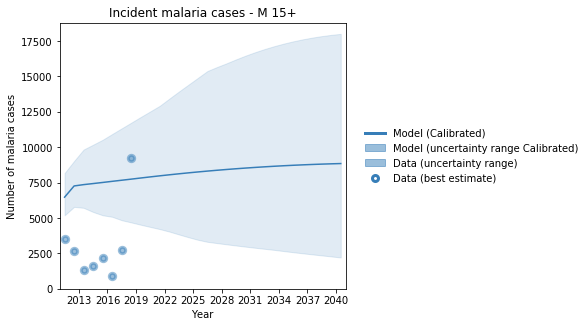
\includegraphics[width=.45\linewidth]{Pursat_high_Incident_M15+.png}} 
\subcaptionbox{Gen, high.\label{Pursat_high_Incident_Gen}}{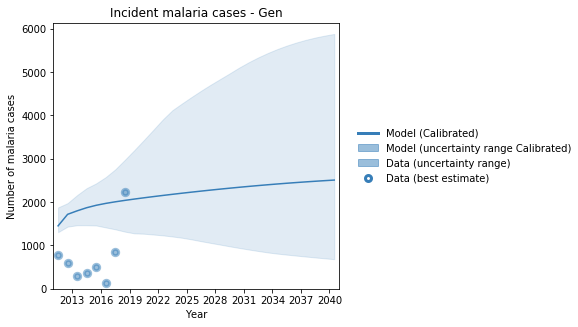
\includegraphics[width=.45\linewidth]{Pursat_high_Incident_Gen.png}} 
\subcaptionbox{M15+, low.\label{Pursat_low_Incident_M15+}}{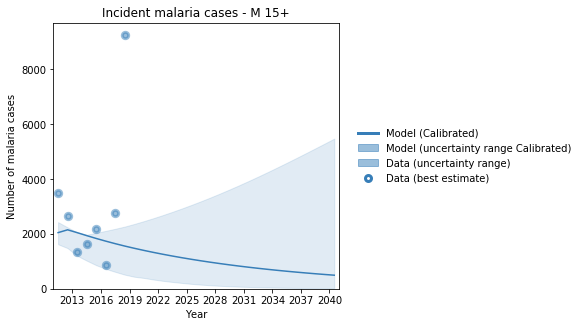
\includegraphics[width=.45\linewidth]{Pursat_low_Incident_M15+.png}} 
\subcaptionbox{Gen, low.\label{Pursat_low_Incident_Gen}}{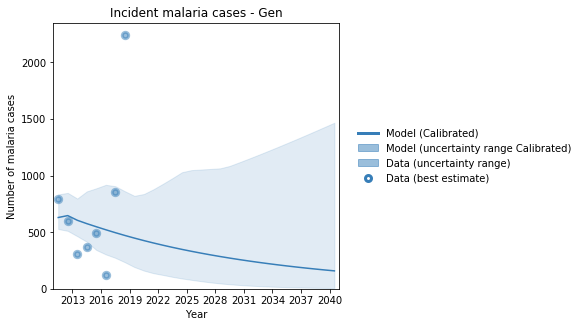
\includegraphics[width=.45\linewidth]{Pursat_low_Incident_Gen.png}} 
\caption{\csentence{Model calibration for Pursat.}}\label{fig:calibration_Pursat}
\end{figure}
\todo{DJP: Fig 2, is there data uncertainty? the legend may not be necessary, or should be less similar to the model uncertainty (I can't see a difference?)}

% -------------- PQ impact figs --------------
\begin{figure}[p]
\centering
\subcaptionbox{M15+, high.\label{Pursat_high_M15+}}{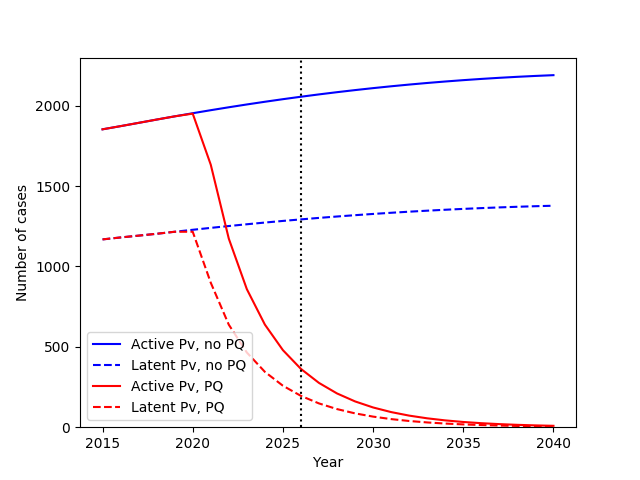
\includegraphics[width=.45\linewidth]{Pursat_high_M15+.png}} 
\subcaptionbox{Gen, high.\label{Pursat_high_Gen}}{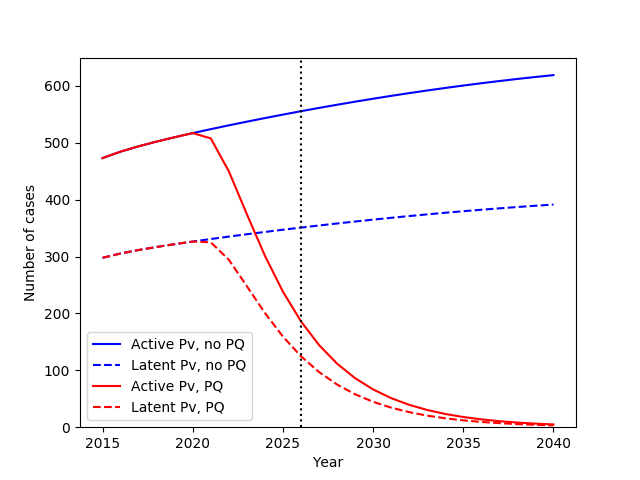
\includegraphics[width=.45\linewidth]{Pursat_high_Gen.png}} 
\subcaptionbox{M15+, low.\label{Pursat_low_M15+}}{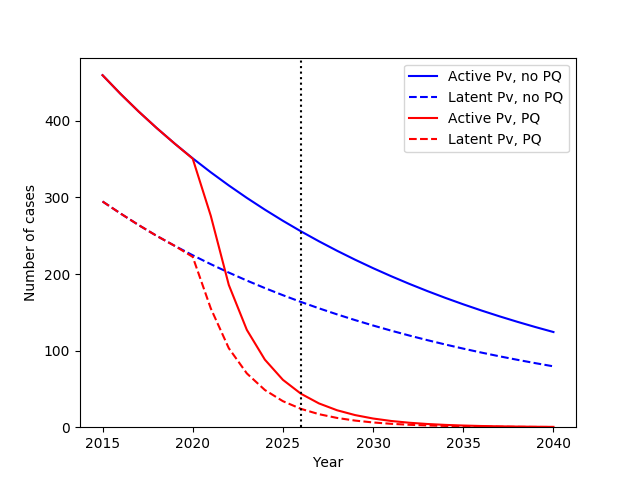
\includegraphics[width=.45\linewidth]{Pursat_low_M15+.png}} 
\subcaptionbox{Gen, low.\label{Pursat_low_Gen}}{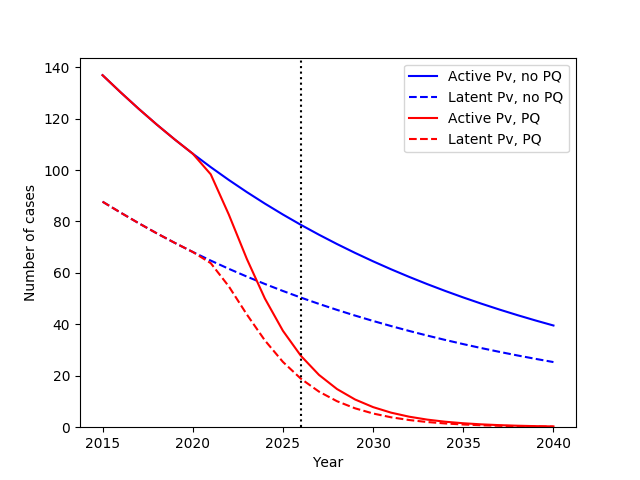
\includegraphics[width=.45\linewidth]{Pursat_low_Gen.png}} 
\caption{\csentence{PQ intervention for \pv~in Pursat.} Vertical dashed line is the current elimination target for \pv.}\label{fig:pq_Pursat}
\end{figure}

\begin{figure}[p]
\centering
\subcaptionbox{M15+, high.\label{Mondulkiri_high_M15+}}{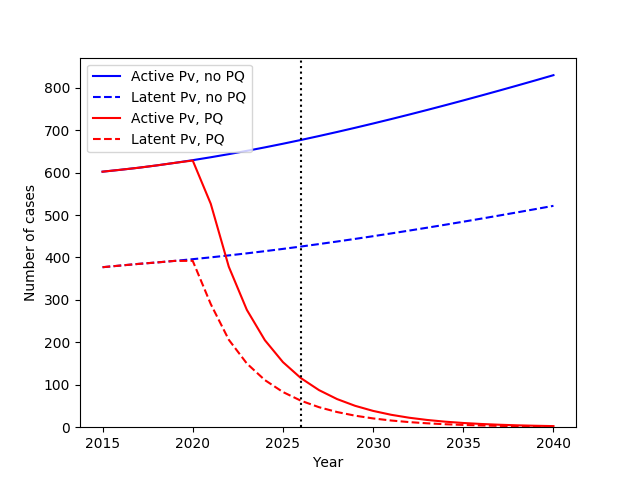
\includegraphics[width=.45\linewidth]{Mondulkiri_high_M15+.png}} 
\subcaptionbox{Gen, high.\label{Mondulkiri_high_Gen}}{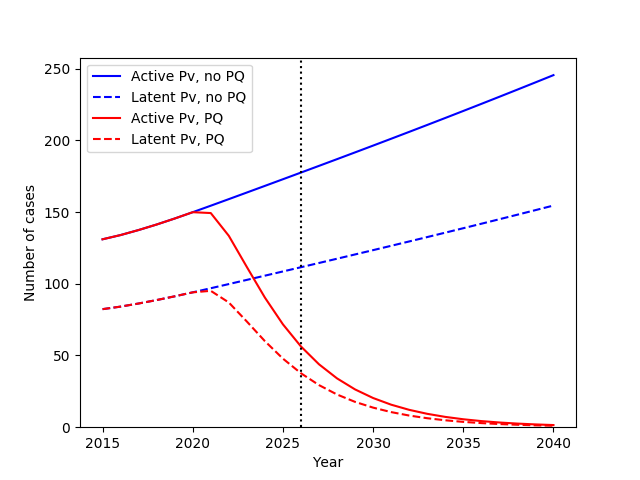
\includegraphics[width=.45\linewidth]{Mondulkiri_high_Gen.png}} 
\subcaptionbox{M15+, low.\label{Mondulkiri_low_M15+}}{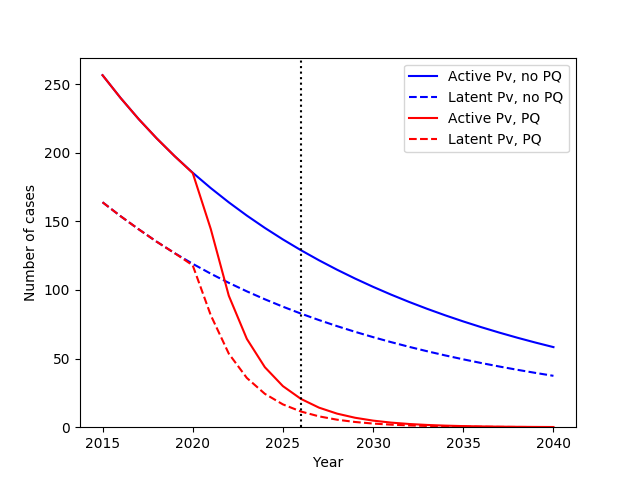
\includegraphics[width=.45\linewidth]{Mondulkiri_low_M15+.png}} 
\subcaptionbox{Gen, low.\label{Mondulkiri_low_Gen}}{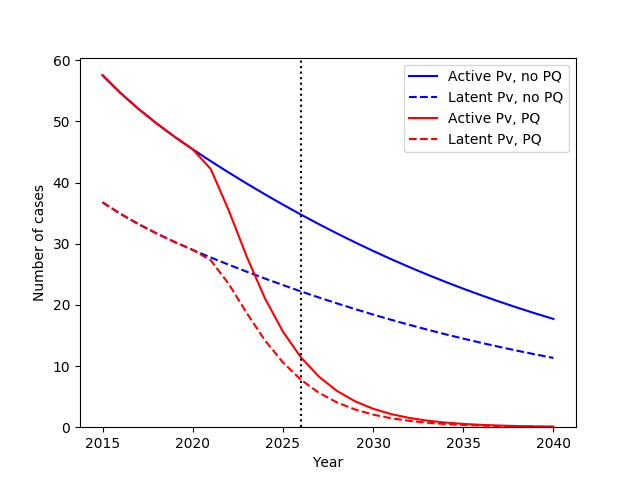
\includegraphics[width=.45\linewidth]{Mondulkiri_low_Gen.png}} 
\caption{\csentence{PQ intervention for \pv~in Mondulkiri.} Vertical dashed line is the current elimination target for \pv.}\label{fig:pq_Mondul_Kiri}
\end{figure}

\begin{figure}[p]
\centering
\subcaptionbox{M15+, high.\label{Kampong_Chhnang_high_M15+}}{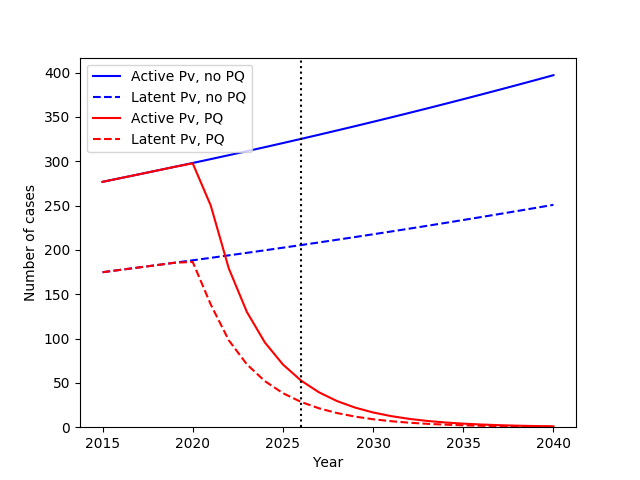
\includegraphics[width=.45\linewidth]{Kampong_Chhnang_high_M15+.png}} 
\subcaptionbox{Gen, high.\label{Kampong_Chhnang_high_Gen}}{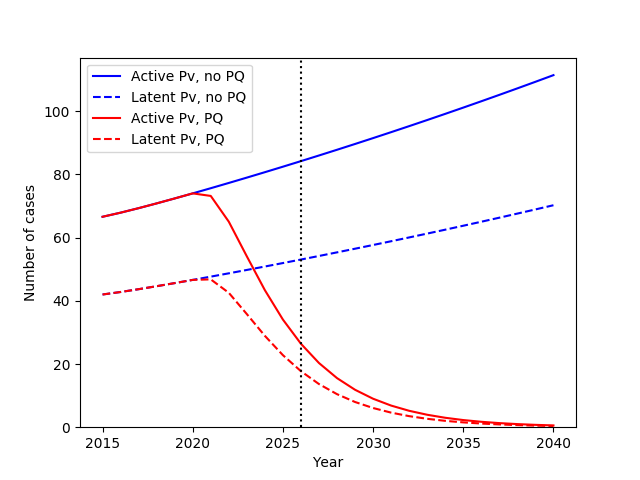
\includegraphics[width=.45\linewidth]{Kampong_Chhnang_high_Gen.png}} 
\subcaptionbox{M15+, low.\label{Kampong_Chhnang_low_M15+}}{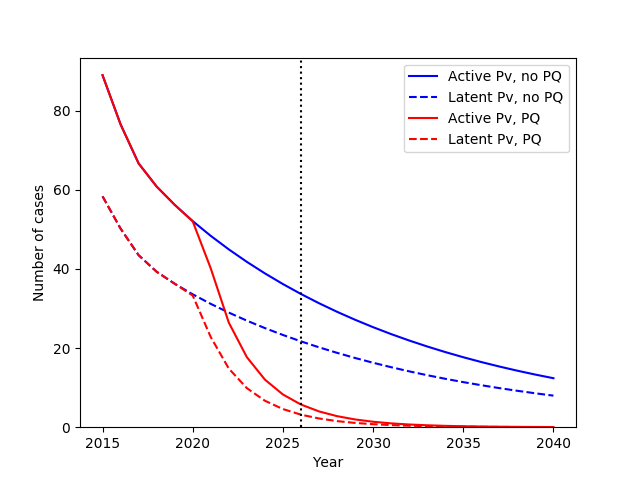
\includegraphics[width=.45\linewidth]{Kampong_Chhnang_low_M15+.png}} 
\subcaptionbox{Gen, low.\label{Kampong_Chhnang_low_Gen}}{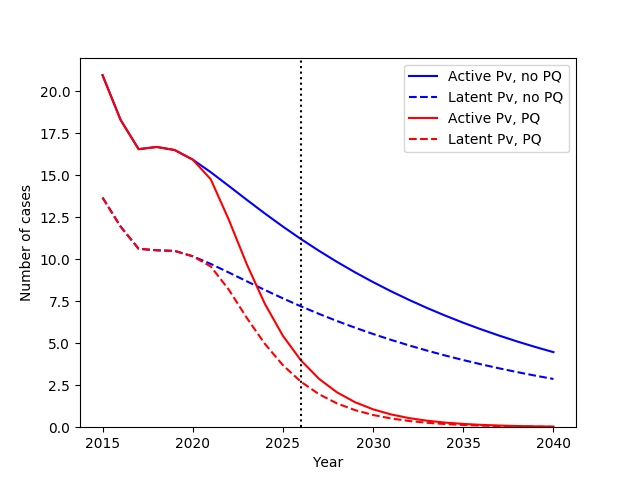
\includegraphics[width=.45\linewidth]{Kampong_Chhnang_low_Gen.png}} 
\caption{\csentence{PQ intervention for \pv~in Kampong Chhnang.} Vertical dashed line is the current elimination target for \pv.}\label{fig:pq_Kampong_Chhnang}
\end{figure}

\begin{figure}[p]
\centering
\subcaptionbox{M15+, high.\label{Battambang_high_M15+}}{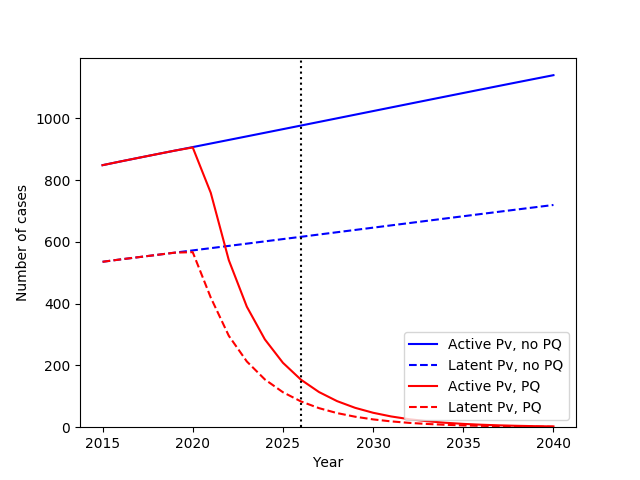
\includegraphics[width=.45\linewidth]{Battambang_high_M15+.png}} 
\subcaptionbox{Gen, high.\label{Battambang_high_Gen}}{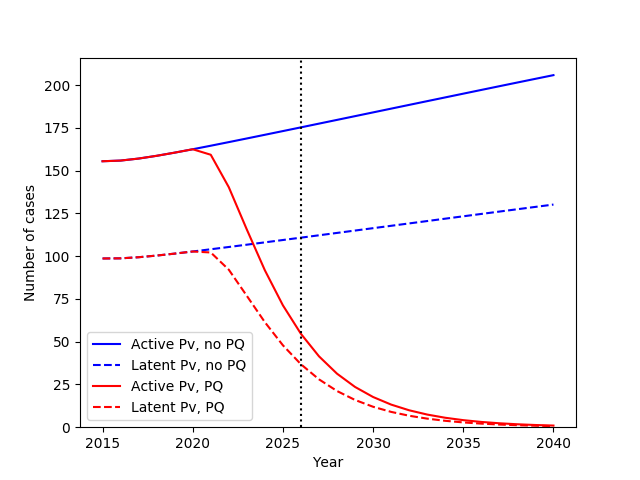
\includegraphics[width=.45\linewidth]{Battambang_high_Gen.png}} 
\subcaptionbox{M15+, low.\label{Battambang_low_M15}}{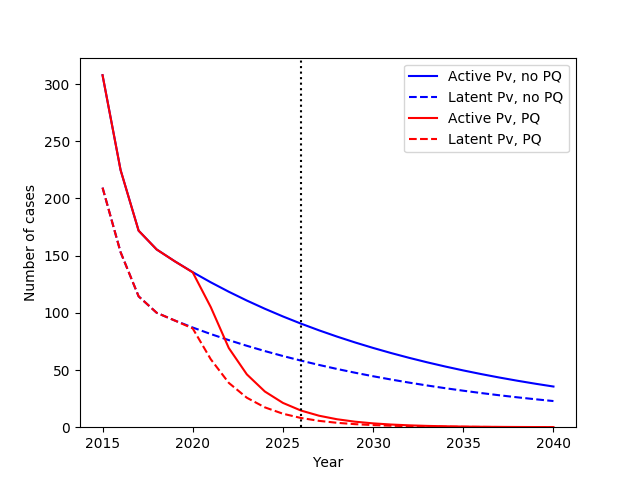
\includegraphics[width=.45\linewidth]{Battambang_low_M15+.png}} 
\subcaptionbox{Gen, low.\label{Battambang_low_Gen}}{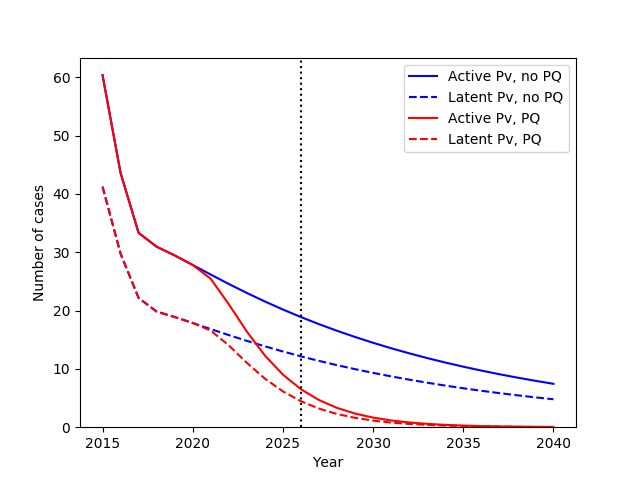
\includegraphics[width=.45\linewidth]{Battambang_low_Gen.png}} 
\caption{\csentence{PQ intervention for \pv~in Battambang.} Vertical dashed line is the current elimination target for \pv.}\label{fig:pq_Battambang}
\end{figure}

\begin{figure}[p]
\centering
\subcaptionbox{M15+, high.\label{Pailin_high_M15+}}{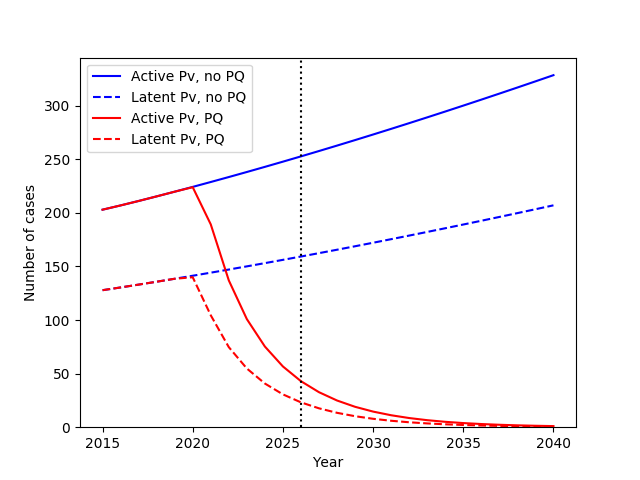
\includegraphics[width=.45\linewidth]{Pailin_high_M15+.png}} 
\subcaptionbox{Gen, high.\label{Pailin_high_Gen}}{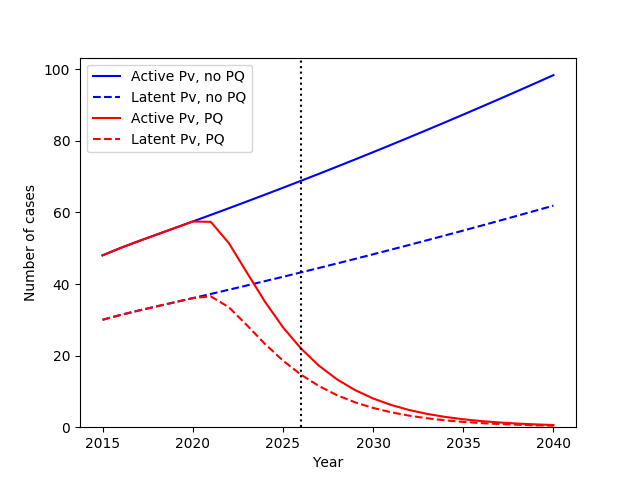
\includegraphics[width=.45\linewidth]{Pailin_high_Gen.png}} 
\subcaptionbox{M15+, low.\label{Pailin_low_M15+}}{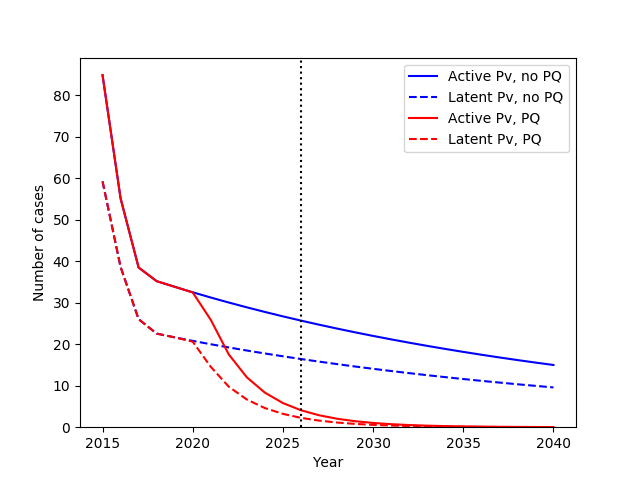
\includegraphics[width=.45\linewidth]{Pailin_low_M15+.png}} 
\subcaptionbox{Gen, low.\label{Pailin_low_Gen}}{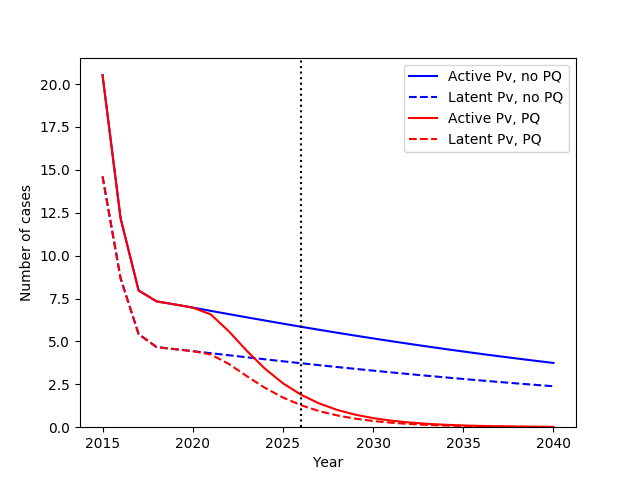
\includegraphics[width=.45\linewidth]{Pailin_low_Gen.png}} 
\caption{\csentence{PQ intervention for \pv~in Pailin.} Vertical dashed line is the current elimination target for \pv.}\label{fig:pq_Pailin}
\end{figure}

\begin{figure}[p]
\centering
\subcaptionbox{M15+, high.\label{Takeo_high_M15+}}{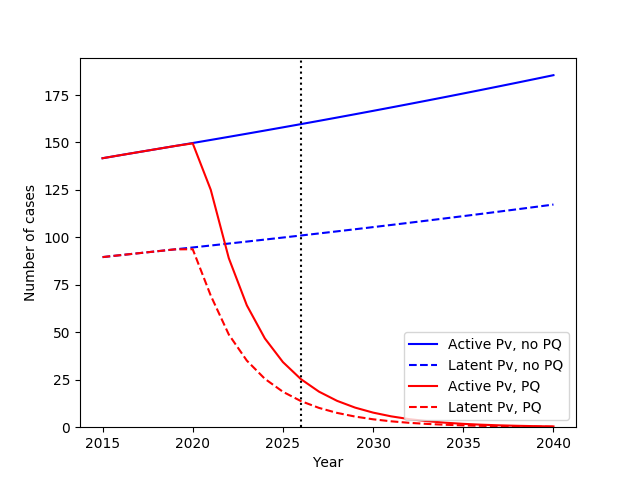
\includegraphics[width=.45\linewidth]{Takeo_high_M15+.png}} 
\subcaptionbox{Gen, high.\label{Takeo_high_Gen}}{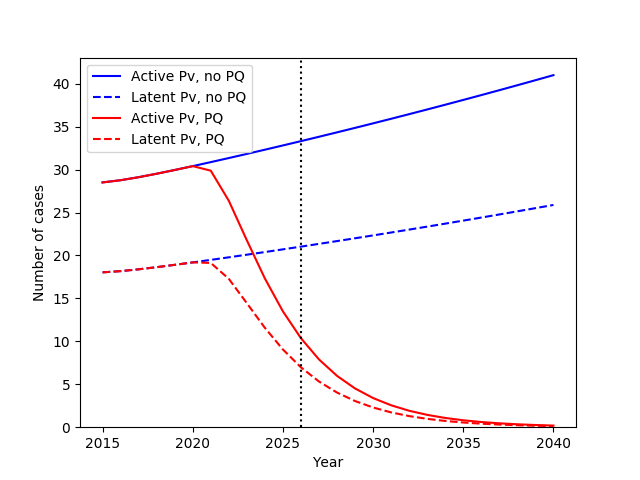
\includegraphics[width=.45\linewidth]{Takeo_high_Gen.png}} 
\subcaptionbox{M15+, low.\label{Takeo_low_M15+}}{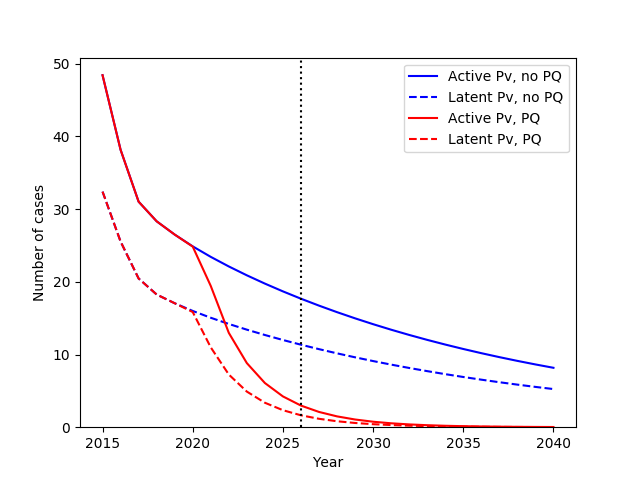
\includegraphics[width=.45\linewidth]{Takeo_low_M15+.png}} 
\subcaptionbox{Gen, low.\label{Takeo_low_Gen}}{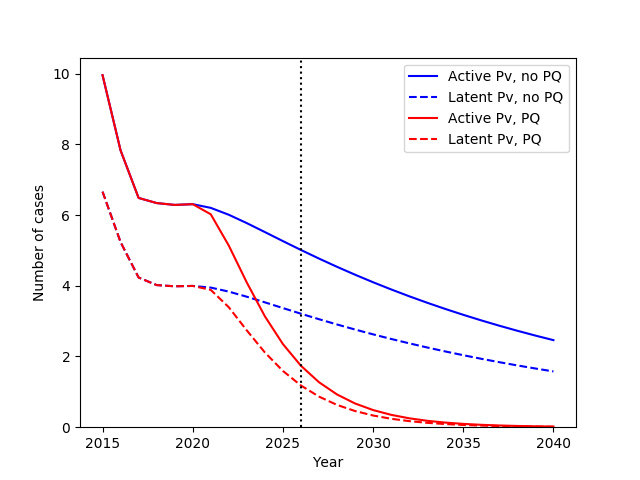
\includegraphics[width=.45\linewidth]{Takeo_low_Gen.png}} 
\caption{\csentence{PQ intervention for \pv~in Takeo.} Vertical dashed line is the current elimination target for \pv.}\label{fig:pq_Takeo}
\end{figure}





%%%%%%%%%%%%%%%%%%%%%%%%%%%%%%%%%%%
%%                               %%
%% Tables                        %%
%%                               %%
%%%%%%%%%%%%%%%%%%%%%%%%%%%%%%%%%%%

%% Use of \listoftables is discouraged.
%%
\section*{Tables}
\begin{table}[p] 
\caption{Surveillance targets for 0.99 probability of detecting at least one case of \pv~in a province, given the scenarios outlined in \S~\ref{sec:methods}, assuming 100\% sensitivity and specificity of the tests (so a lower bound on number of targets).}\label{tab:surveillance}
      \begin{tabular}{|l|l|l|l|l|l|l|l|l|l|}
       \hline 
       \multicolumn{2}{|l|}{Year} & \multicolumn{4}{|c|}{2020} & \multicolumn{4}{|c|}{2025} \\ \hline
       \multirow{2}{*}{Scenario} & Incidence & Low & Low & High & High & Low & Low & High & High \\ %\hline 
                                 & Primaquine & None & M 15+ & None & M 15+ & None & M 15+ & None & M 15+ \\ \hline
    \multirow{6}{*}{Province} & Pursat & 441 & 444 & 2,345 & 76 & 76 & 557 & 2,610 & 70 \\ %\hline
                              & Mondulkiri & 172 & 173 & 48 & 48 & 280 & 1,388 & 54 & 263 \\ %\hline
                              & Kampong Chhnang & 3,798 & 3,819 & 649 & 653 & 5,564 & 26,094 & 614 & 2,998 \\ %\hline 
                              & Battambang & 2,962 & 2,978 & 433 & 436 & 3,916 & 19,191 & 384 & 1,922 \\ %\hline
                              & Pailin & 850 & 855 & 123 & 124 & 1,040 & 4,960 & 122 & 579 \\ %\hline 
                              & Takeo & 14,335 & 14,415 & 2,345 & 2,358 & 18,905 & 89,418 & 2,205 & 10,919 \\ \hline 
      \end{tabular}
\end{table}

%%%%%%%%%%%%%%%%%%%%%%%%%%%%%%%%%%%
%%                               %%
%% Additional Files              %%
%%                               %%
%%%%%%%%%%%%%%%%%%%%%%%%%%%%%%%%%%%

\section*{Additional Files}
%  \subsection*{Additional file 1 --- Sample additional file title}
%    Additional file descriptions text (including details of how to
%    view the file, if it is in a non-standard format or the file extension).  This might
%    refer to a multi-page table or a figure.
%
%  \subsection*{Additional file 2 --- Sample additional file title}
%    Additional file descriptions text.

\subsection*{Additional file 1 --- Model and data details}
    Detailed descriptions of the model and data are provided here, including supplementary figures with a further breakdown on the modelled impact. 


\end{backmatter}
\end{document}
